\chapter{Experimental Results} % (fold)
\label{cha:experiments}

This chapter presents the experimental work completed to validate the actuator dynamics and motion control framework. It is important to test walking control strategies on physical hardware directly due to the imperfections in a simulation environment. For example, the contact models used to estimate the ground reaction force is only an approximation. There are also other unmodeled effects which can significantly alter the dynamics of the physical system (i.e. vibrations). The simulations used to demonstrate the proposed 3D FPE walking control strategy in the previous section accounted for link side dynamics only. Section~\ref{sec:actuator_model} describes the modifications to account for the actuator dynamics. This modification to the simulations enables a single controller designed in Simulink to target either the simulation environment or the physical hardware using the HIL architecture discussed in Section~\ref{sec:hil_architecture}. The experimental validation for a single actuator and the proposed motion control framework are presented in Sections \ref{sec:1dof_validation} and \ref{sec:motion_control_validation}, respectively. 

\section{Actuator Model} % (fold)
\label{sec:actuator_model}
PD control is applied for each joint in order to track the desired trajectory generated by higher levels of control (Section~\ref{sub:control_strategy}). The control signal $u$ produced at each joint $k$ is provided by (where $k = 1 \ldots n$ is the $k$-th joint of the $n$-DOF system) : 

\begin{equation}
	{u_k} = {K_P}({q_{d_k}} - {q_k}) - {K_D}{\dot q_k}
	\label{eq:pdcontrollaw}
\end{equation} 

Where ${q_{d_k}}$ and ${q_k}$ are the desired and actual angles and ${\dot q_k}$ is the velocity of the $k$-th joint. Constants ${K_P}$ and ${K_D}$ are the porportional and derivative gains of the controller, respectively. In the ideal case, the control signal ${u_k}$ would simply be applied torque ${\tau _k}$ to each joint from $\vtau = \left[\tau _1 \ldots \tau _k \right]$ shown on the right hand side of (\ref{eq:eom1}). However, the actuator dynamics of DC motors used in the development of the 14 DOF bipedal robot must be considered. The motors selected in Section~\ref{sub:final_configurations} are controlled by a voltage control signal $v_{m}$. A second order system is used to model the actuator dynamics and relate the applied torque to the motor voltage $v _m$ \cite{Spong2008}: 

\begin{equation}
	{J_m}{\ddot \Theta _m} + \left( {{B_m} + \frac{{{k_b}{k_m}}}{{{r_a}}}} \right)\dot \Theta _m  = {\tau _m} - \frac{{{\tau _l}}}{{{g_r}}}
	\label{eq:actdyn1}
\end{equation}

Where $\Theta _m$ is the rotor angle, $J_m$ is the motor inertia, $B_m$ is the motor damping, $k_b$ is the back emf or voltage constant, $k_m$ is the torque constant, $r_a$ is the armature resistance and $g_r$ is the gear reduction ratio. The motor torque $\tau _m$ is related to the (link side) load torque $\tau _l$ through the gearing ratio $g_r$. Since the output side of the gearhead is coupled directly to the link, the motor angles are related to the joint angles by: 

\begin{equation}
	{\Theta _{m_k}} = {g _{r_k}} {q _k}
	\label{eq:actdyn2} 
\end{equation}

Similarly, the joint torques in $\vtau$ (\ref{eq:eom1}) are related to the actuator load torques by: 

\begin{equation}
	{\tau _{m_k}} = {\frac{\tau _{k}}{g _{r_k}}} 
	\label{eq:actdyn3}
\end{equation}

Furthermore, the motor torque is related to the applied voltage through the following relationship: 

\begin{equation}
	{\tau _{m_k}} = {k_m} {i_a} = \left( {\frac{{{k_m}}}{{{r_a}}}} \right){v _{m_k}}
	\label{eq:actdyn4}
\end{equation}


Where $i_a$ is the current through the armature wiring. Substituting equations (\ref{eq:actdyn2} - \ref{eq:actdyn4}) back into (\ref{eq:actdyn1}) yields the complete relationship between the $k$-th joint angle, link side torque and the applied motor voltage:

\begin{equation}
	g_r^2{J_m}{\ddot q_k} + g_r^2\left( {{B_m} + \frac{{{k_b}{k_m}}}{{{r_a}}}} \right){\dot q_k} = g_r^{}\left( {\frac{{{k_m}}}{{{r_a}}}} \right){v_k} - {\tau _k}
	\label{eq:actdyn5}
\end{equation}

Note that the drivetrain constants specific to the $k$-th joint are used (i.e. ${J _{m_k}}$, ${B _{m_k}}$, $g _{r_k}$, etc.) in this equation (\ref{eq:actdyn5}). 

\subsection{Independent Joint Control} % (fold)
\label{sub:independent_joint_control}

% subsection independent_joint_control (end)

Using independent joint control \cite{Sciavicco2001}, each joint $k$ of the system is decoupled from the rest of the system and controlled individually. The control signal for each joint is computed directly from its own reference trajectory, position and velocity. This approach does not account for the coupled dynamics of the overall system described by (\ref{eq:eom1}). The link side torques in (\ref{eq:actdyn5}) are treated as a disturbance to the second order system and the motor inertia and damping are modified as follows: 

\begin{equation}
	\begin{array}{l}
		{J_{eff}} = g_r^2{J_m} + {a_{kk}}\\
		{B_{eff}} = g_r^2({B_m} + {k_b}{k_m}/{r_a})
	\end{array}
	\label{eq:actdyn6}
\end{equation}

Where ${J_{eff}}$ and ${B_{eff}}$ are the effective motor inertia and damping \emph{seen} by the joint. The ${a_{kk}}$ in (\ref{eq:actdyn6}) compensates for the inertia of link $k$ by adding the $k$-th diagonal term from the inertia matrix $A(\vec{q})$ in (\ref{eq:eom1}). Substituting back into (\ref{eq:actdyn5}) yields: 

\begin{equation}
	{J_{eff}}{\ddot q_k} + {B_{eff}}{\dot q_k} = g_r^{}\left( {\frac{{{k_m}}}{{{r_a}}}} \right){v_k} - {d_k}
	\label{eq:actdyn7}
\end{equation}

Where ${d_k} = \tau _k$ is the link side torque treated as a disturbance to the system. Taking the control input $u _k$ (\ref{eq:pdcontrollaw}) to be the voltage signal $v _m$ in (\ref{eq:actdyn7}) yields a closed loop controller for independent joint control with actuator dynamics (implemented in Figure~\ref{fig:pdmotorcontroller}).

\begin{figure}[!h]
	\centering
    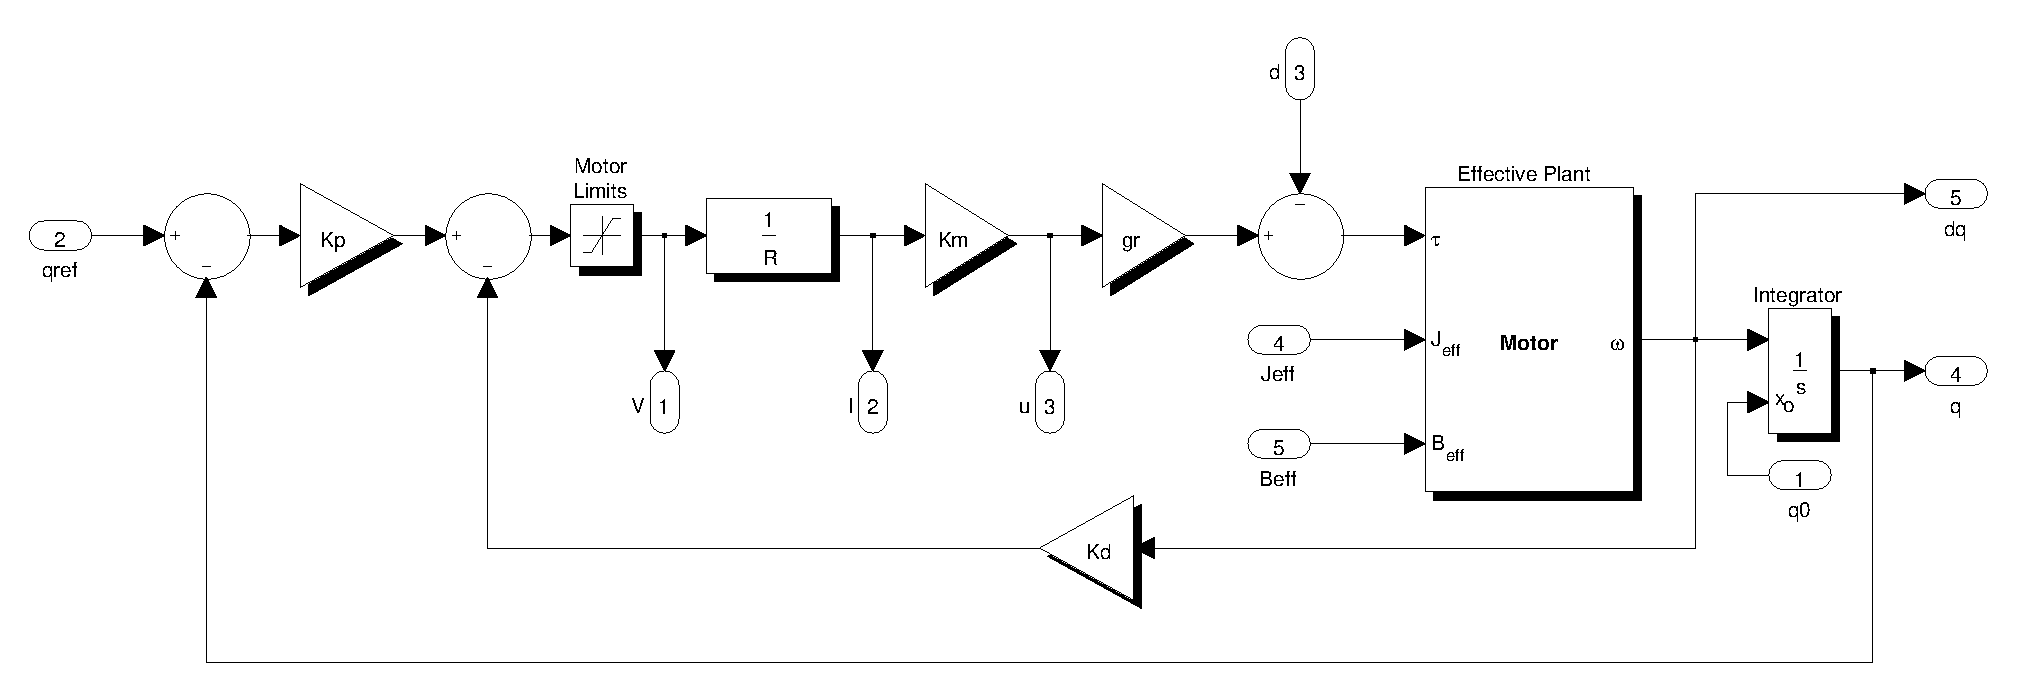
\includegraphics[scale=0.5]{fig/experiments/pdmotorcontroller.eps} 
  	\caption{PD Controller implementation for independent joint control with actuator dynamics.}
	\label{fig:pdmotorcontroller}
\end{figure}

To improve the estimate of the motor side inertia, $a_{kk}$ is required in (\ref{eq:actdyn6}). The dynamic simulation package used in Section~\ref{sec:simulations_and_results} is based on Mathwork's Simulink environment and uses the SimMechanics toolbox which does not allow the mass matrix $A(\vec{q})$ to be isolated. Therefore, the following algorithm was used to compute the mass matrix and extract the diagonal terms at each time step: 

\begin{algorithm}[H]
 \SetAlgoLined
 Initialization\;
 Set $\vec{q} = \vec{q}_0$, $\vec{\dot q} = \vec{\dot q}_0$, $\vec{\ddot q} = \vec{0}$\;
 \While{1}{
  Compute $\hat{\vtau}$ using RNE with $\vec{\ddot q} = \vec{0}$\;
  \For{$i = 1$ to $n$}{
  Set $\tilde{\vec{g}} = \vec{0}$, $\mathbf{\tilde{\dot{q}}} = \vec{0}$, $\mathbf{\tilde{\ddot{q_i}}} = 1$, $\mathbf{\tilde{\ddot{q_j}}} = 0$ $[j \ne i]$\;
  Compute $\tilde{\vtau}$ using RNE\;
  Form $i$-th column: $A(\vec{q})_{i} = \tilde{\vtau} - \hat{\vtau}$
  }
  Combine columns to form $A(\vec{q})$\;
  Select diagonal elements of $A(\vec{q})$\;
 }
 \caption{Computing mass matrix diagonal terms with RNE algorithm}
 \label{alg:massdiag}
\end{algorithm}

% section actuator_model (end)

\section{HIL Architecture} % (fold)
\label{sec:hil_architecture}
The architecture used to control the physical 14 DOF bipedal robot is presented in this section. In general, controlling DC motors requires a controller (to host the control algorithm) and a driver (typically serves as a power amplifier). The controller outputs a low voltage control signal which is amplified by the driver and applied to the terminals of the motor. Encoders are used to sense the rotor position information and passed back to the controller for closed loop  control. 

The physical hardware developed in Chapter~\ref{cha:design} is treated as the plant. Using Quanser's QUARC toolbox, control algorithms developed in the Simulink environment can be compiled for a variety of target platforms ranging from embedded microcontrollers to standard PC. This allows the use of a shared codebase for simulation and for the physical hardware. The control algorithms used for the biped are compiled and executed on a PC which communicates with the physical hardware through a data acquisition (DAQ) board. A separate and dedicated voltage amplifier is used to drive the DC motors from a low voltage analog control signal (labeled ``amplifier command'' on Figure~\ref{fig:hilarch}) from the controller via the DAQ. 

\begin{figure}[!h]
	\centering
    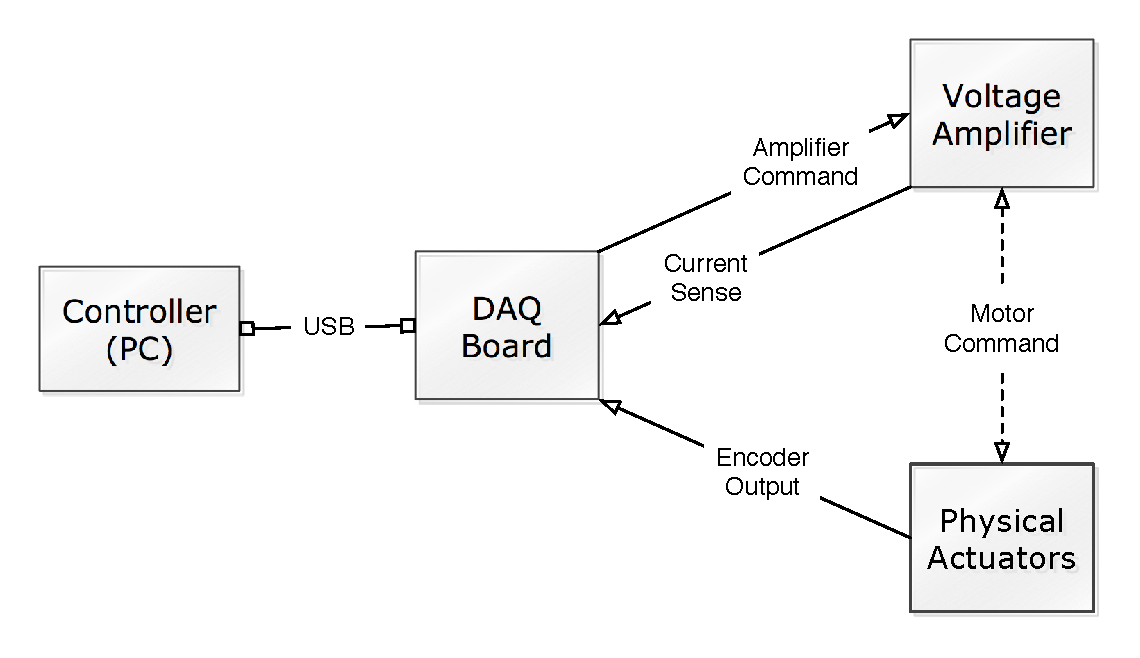
\includegraphics[scale=0.65]{fig/experiments/hilarchitecture.eps} 
  	\caption{Hardware architecture used to control the physical 14 DOF bipedal robot.}
	\label{fig:hilarch}
\end{figure}

The actuator subassemblies selected in Section~\ref{sub:final_configurations} were preassembled with incremental optical encoders mounted to the motor side. These encoders output digital signals on two channels for an indication and control of the motor shaft position and direction.  These digital signals are passed back to the controller running on the PC via the DAQ. Using quadrature decoding, the motor angle $\Theta _m$ and velocity $\dot{\Theta}_m$ can be retrieved from the encoder output in degrees: 

\begin{equation}
	{\Theta _m} = \frac{{360}}{{n \cdot l}} \cdot Encoder_{output}
\end{equation}

Where $n = 4$ for quadrature (4X) decoding and $l$ is the lines per revolution specified from the encoder manufacturer. Using the relationship between the motor variables and the joint variables in (\ref{eq:actdyn2}), an estimate of the $k$-th link side angle (at the output of the gearhead) can be obtained: 

\begin{equation}
	{q_k} = \frac{{360}}{{4 \cdot l \cdot {g_{{r_k}}}}} \cdot Encode{r_k}
	\label{eq:quadrature}
\end{equation}

This is only an estimate of the joint angle since there are drivetrain losses (i.e. in the gearhead) which are ignored by an encoder mounted to the motor side. 

\subsection{Parallel Models} % (fold)
\label{sub:parallel_models}

The ability to develop a single controller and target either a simulation environment or the physical hardware is extremely useful. Using the Quanser's QUARC toolbox, a Q8-USB (DAQ) board and a VoltPAQ (voltage amplifier), the control algorithms were redeveloped as parallel models capable of switching target platforms (shown in Figure~\ref{fig:parallelmodels}).

\begin{figure}[!h]
	\centering
    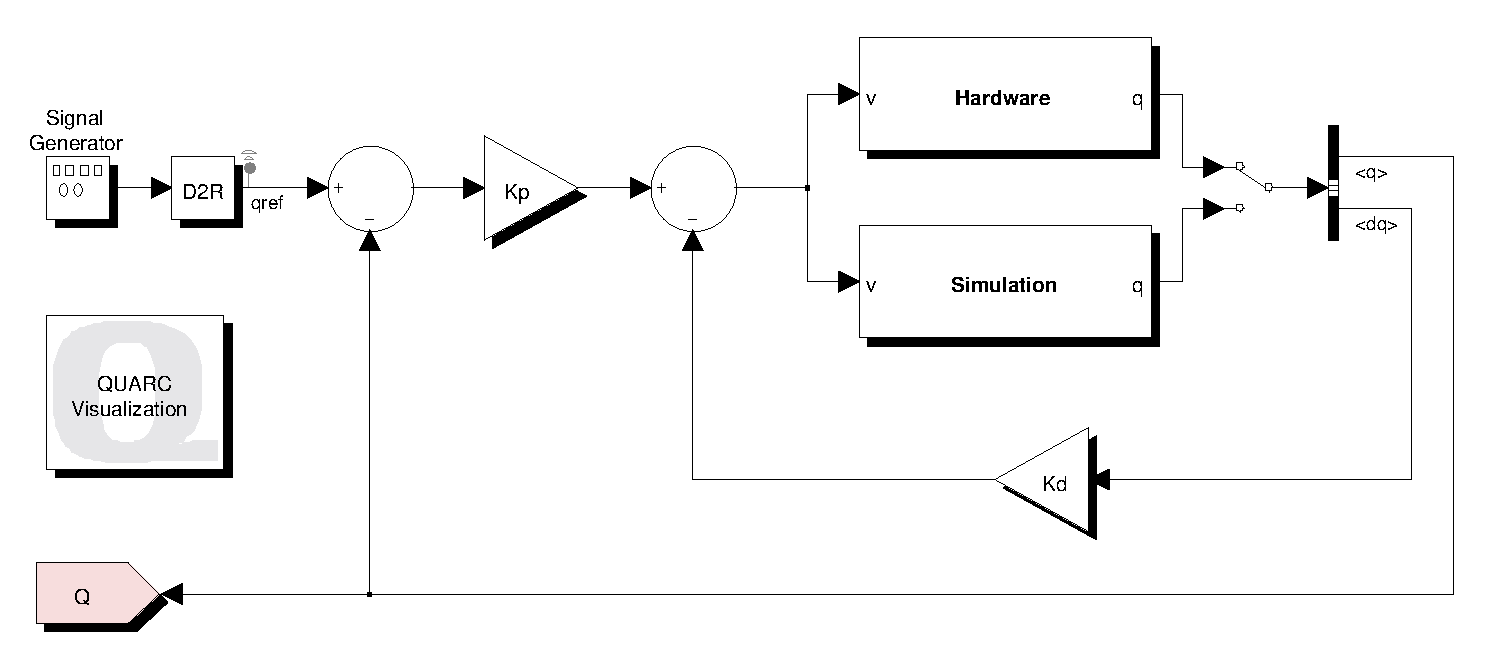
\includegraphics[scale=0.6]{fig/experiments/parallelmodels.eps} 
  	\caption{Parallel models designed to target either simulations or physical hardware with the same controller.}
	\label{fig:parallelmodels}
\end{figure}

In the physical environment mode shown in Figure~\ref{fig:hilmodel}, the hardware target subsystem is initialized to interface with the Q8-USB DAQ board. The control algorithm running on the PC communicates with the physical hardware using ``HIL Read'' and ``HIL Write'' blocks which communicate with the DAQ over USB. The PD controller output is an analog signal corresponding to the desired voltage at the motor terminals (amplifier command). The DAQ also reads the raw digital signals from the motor side encoders. The VoltPAQ voltage amplifier also provides the ability to read the current in the armature circuit ($i_a$) of the DC motor. This value is passed back to the controller through the DAQ using an analog channel. Due to the noise in the current sensor, a low pass filter is used to produce a cleaner signal. The quadrature decoding formula (\ref{eq:quadrature}) is used to obtain the joint angle for the closed loop feedback. The link side angle information is also used to determine whether a joint is out of its limits. The controller detects and sends a ``shut down'' command to the amplifier channel if it is. 

\begin{figure}[!h]
	\centering
    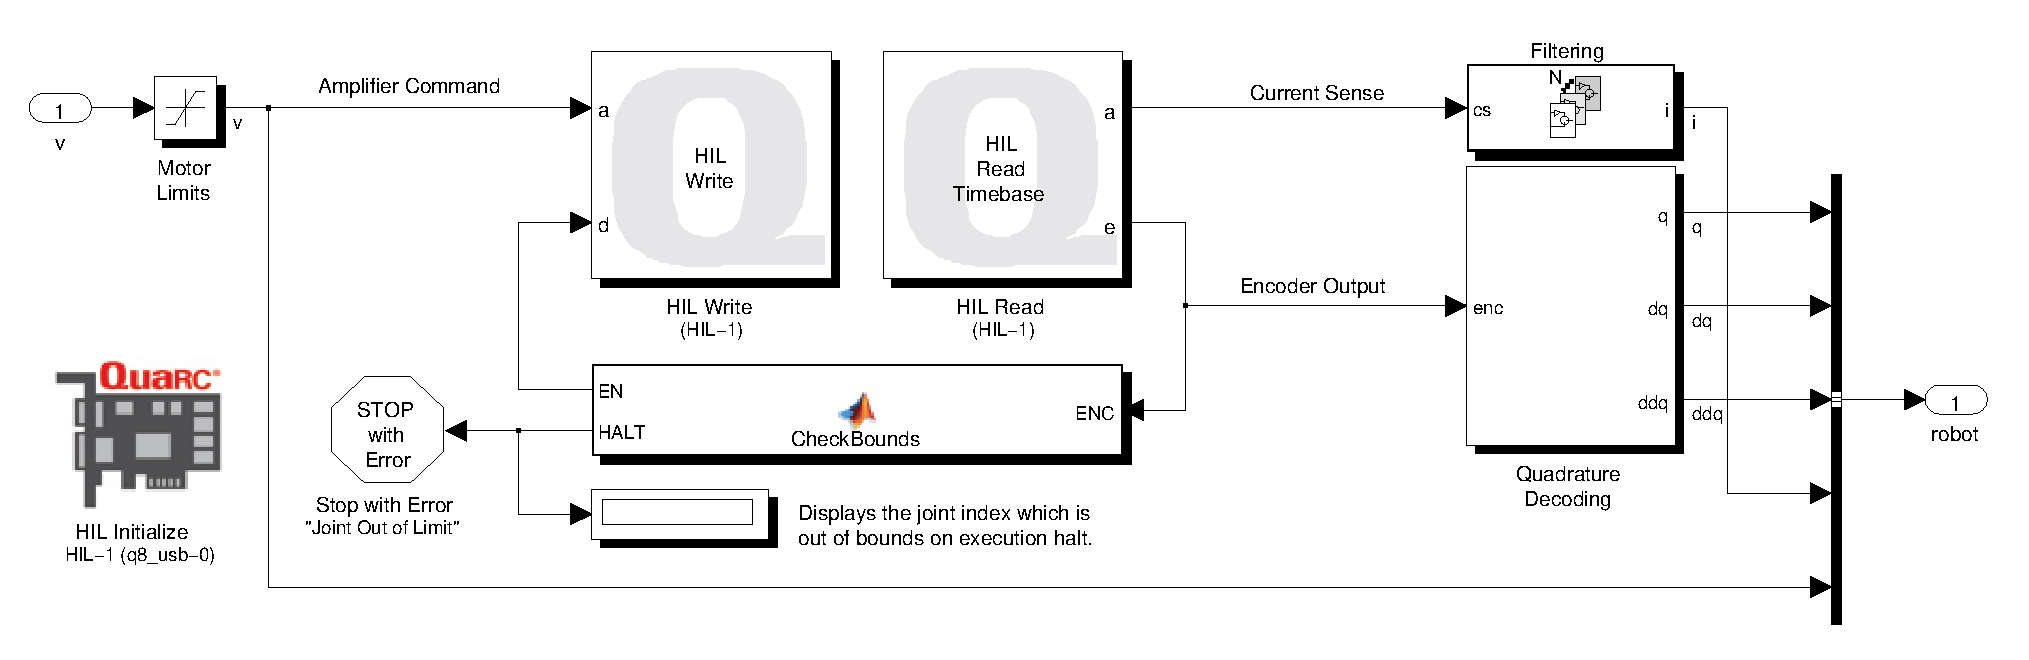
\includegraphics[scale=0.45]{fig/experiments/hilmodel.eps} 
  	\caption{HIL subsystem from Figure~\ref{fig:parallelmodels} used to target physical hardware with voltage control signal.}
	\label{fig:hilmodel}
\end{figure}

In the simulated environment mode, the controllers were reformulated to use the voltage signal as the control input. The actuator dynamics were incorporated into the simulation using the independent joint control formulation presented in (\ref{eq:actdyn7}). The simulation target subsystem shown in Figure~\ref{fig:simmodel} computes the effective motor inertia and damping seen by the joint using Algorithm~\ref{alg:massdiag}. The link side joint angle, velocity and accelerations are used with inverse dynamics to compute the link side torque which is treated as a disturbance to the system. 

\begin{figure}[!h]
	\centering
    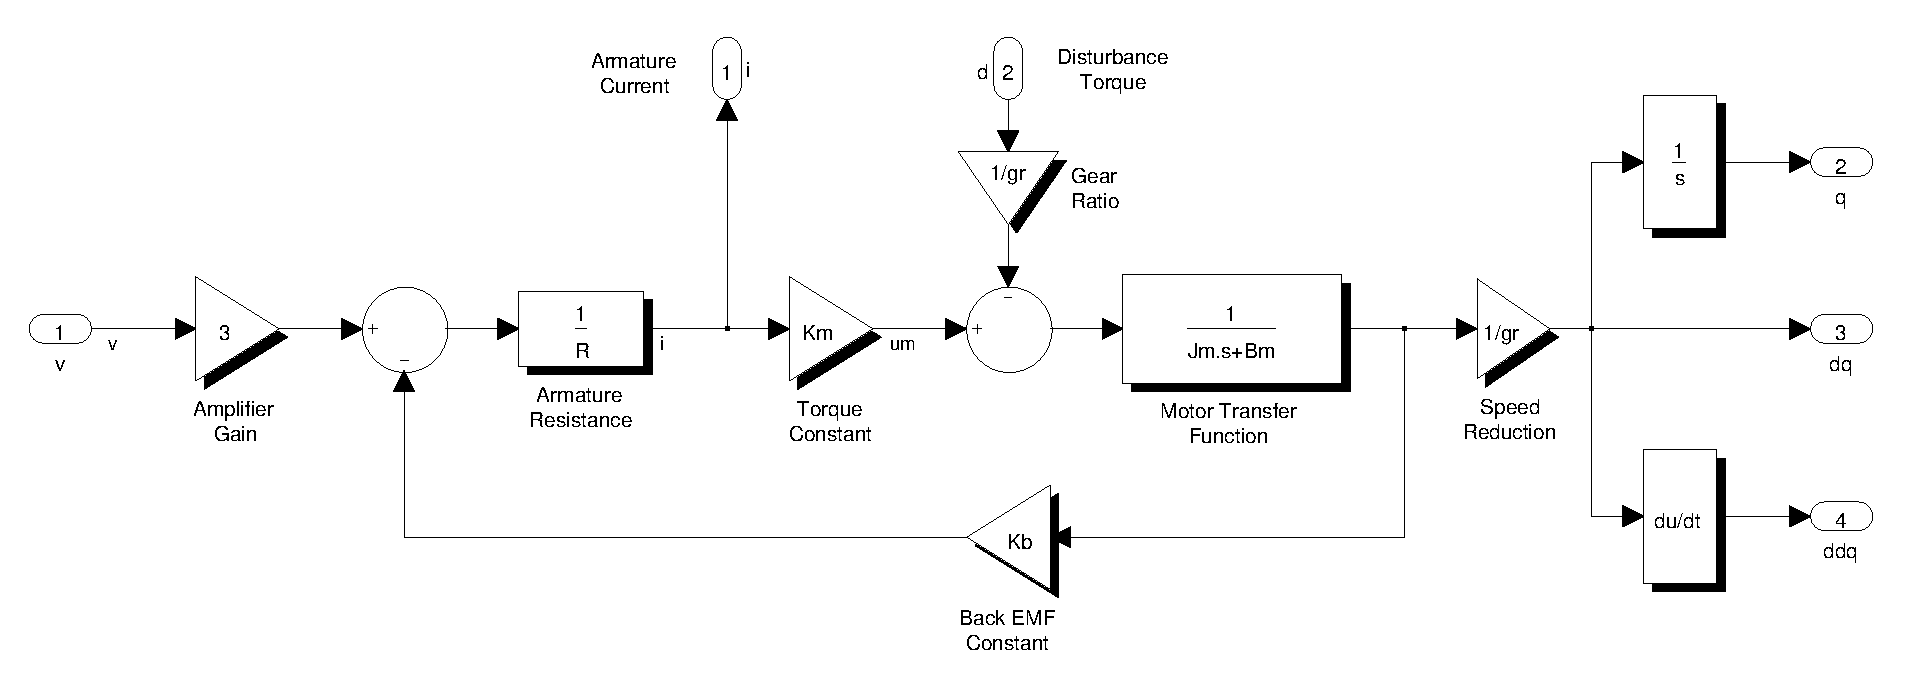
\includegraphics[scale=0.55]{fig/experiments/simmodel.eps} 
  	\caption{Subsystem from Figure~\ref{fig:parallelmodels} used to target the simulated environment with voltage control signal.}
	\label{fig:simmodel}
\end{figure}


% subsection parallel_models (end)

% section hil_architecture (end)

\section{Single DOF Validation} % (fold)
\label{sec:1dof_validation}
This section describes the experiments validating the simulation models for 1 DOF controllers using the HIL environment. 

\subsection{Joint Tracking} % (fold)
\label{sub:joint_tracking}
The parallel model for targetting the simulation environment and physical hardware was used to tune the PD controller gains for a single joint of the bipedal robot. By using the shared controller architecture, gains were tuned to improve tracking performance in the simulation environment and then immediately verified on the physical hardware. The experimental results presented in this section show the results of the hip yaw joint tracking a sine wave at 0.5 Hz with a $15^{\circ}$ amplitude.

\begin{figure}[!h]
	\begin{center}
	\subfigure{\includegraphics[scale=0.45]{fig/experiments/simtrack1dof.eps}}
	\subfigure{\includegraphics[scale=0.45]{fig/experiments/hiltrack1dof.eps}}
	\end{center}
  	\caption{Single joint tracking results shown in simulation (left) and hardware (right).}
	\label{fig:tracking1dof}
\end{figure} 

The tracking results shown in Figure~\ref{fig:tracking1dof} validate the simulation models. The same controller gains were used on the physical hardware and the tracking performance is almost identical to the simulated case.   
% subsection joint_tracking (end)

\Incomplete
% section 1dof_results (end)

\section{Motion Control Validation} % (fold)
\label{sec:motion_control_validation}
\Incomplete
% section motion_control_results (end)

\section{Discussion} % (fold)
\label{sec:experiments_discussion}
Validating control algorithms on physical hardware is important due to modeling imperfections in the simulation environment. The physical 14 DOF bipedal robot developed in earlier chapters was used for experimental validation through HIL testing. 

For the physical hardware, DC motors are controlled by a voltage signal $v_m$. A second order system was used to model the actuator dynamics and reformulate the existing controllers which controlled the link side torques $\tau _k$. Independent joint control decouples each joint for individual control. Since this approach does not account for the coupled dynamics of the overall system, the link side torques are treated as a disturbance to the actuator dynamics model. The effective motor inertia is reformulated to include the link inertia seen by the joint. A generic RNE-based algorithm was used to extract the mass matrix of the system at every time step to compute the effective motor inertia.

The HIL architecture was developed using Quanser's QUARC toolbox, DAQ board and a voltage amplifier. The controller code developed in Simulink was targetted to execute on the PC. The DAQ board allowed the PC-based controller to communicate with the physical hardware through analog and digital I/O. Quadrature decoding was on the encoder output to obtain the link side joint angles on physical hardware for closed loop feedback control. Parallel simulation models were developed for experimental validation to target the physical hardware or the simulated actuator dynamics. 

The single DOF simulations were demonstrated on physical hardware. The simulated environment was used to tune the PD gains for the physical hardware. It was shown that tracking performance of the PD controller was identical in both environments.  

\Incomplete
% section discussion (end)

% chapter experiments (end)